\documentclass[a4paper, 11pt]{article}

% Nécessaire
\usepackage[french]{babel}
\usepackage[utf8]{inputenc}
\usepackage[T1]{fontenc}
\usepackage{lmodern}
\usepackage{amsmath, amsthm}
\usepackage{amsfonts,amssymb}

% Marge
\usepackage{geometry}
\geometry{margin={2.2cm ,2cm}}

% Figures, graphiques
\usepackage{graphicx}
\usepackage{epsfig}
\usepackage{caption}

% Surlignage
\usepackage{alltt}

\usepackage{xcolor}
\usepackage{soul}
\usepackage{color}
\usepackage{colortbl}

% Indicatrice
\usepackage{dsfont}

\usepackage{multirow}
\usepackage{eurosym}
\usepackage{extarrows}


% Titre
\title{Modification des échanges de cécidomyies entre les sous-blocs}
\author{}
\date{}



\begin{document}
\maketitle 

Ce document détaille et illustre les changements induits par la modification des échanges de femelles entre les trois sous-blocs.

\section{Ce qui change}

\paragraph{Ancienne hypothèse} Les cécidomyies quittent le sous-bloc duquel elles émergent avec une probabilité $p_m$. La proportion $p_m$ de cécidomyies qui quittent le sous-bloc $i$ s'en va exclusivement dans les sous-blocs $j$ et $k$, proportionnellement aux inflorescences de ces deux sous-blocs. Ainsi, si l'on note $N^{\text{endo}}_{t, i}$ le nombre de femelles émergeant dans le sous-bloc $i$ à la date $t$, on obtient que :
\begin{itemize}
 \item $(1-p_m)N^{\text{endo}}_{t, i}$ femelles restent dans le sous-bloc $i$;
 \item $p_m \frac{I_{t, j}}{I_{t, j} + I_{t, k}}N^{\text{endo}}_{t, i}$ femelles s'en vont dans le sous-bloc $j$;
 \item $p_m \frac{I_{t, k}}{I_{t, j} + I_{t, k}}N^{\text{endo}}_{t, i}$ femelles s'en vont dans le sous-bloc $k$.
\end{itemize}

\paragraph{Nouvelle hypothèse} Les femelles quittant les sous-blocs ayant un enherbement ras ou haut s'en vont exclusivement vers le sous-bloc baché (\textit{i.e.} l'unique sous-bloc limitrophe).
On émet l'hypothèse qu'il y a au moins toujours une proportion $\frac{I_{t, i}}{I_{t, i} + I_{t, \text{PS}}}$ de femelles qui reste dans le sous-bloc $i$ (avec $i \in \{\text{ER, EH}\}$). Parmi les $\frac{I_{t, \text{PS}}}{I_{t, i} + I_{t, \text{PS}}} N^{\text{endo}}_{t, i}$ femelles restantes, toutes ne s'en vont pas dans le sous-bloc baché : il y a un coût lié au départ du sous-bloc (cela se traduit par le fait qu'une cécidomyie n'a pas d'intérêt à migrer si elle dispose de ressources là où elle émerge). Au final, on a :
\begin{itemize}
 \item $\left(\frac{I_{t, i}}{I_{t, i} + I_{t, \text{PS}}} + (1-p_{\text{PS}})\frac{I_{t, \text{PS}}}{I_{t, i} + I_{t, \text{PS}}}\right) N^{\text{endo}}_{t, i}$ femelles qui restent dans le sous-bloc $i$;
 \item $p_{\text{PS}}\frac{I_{t, \text{PS}}}{I_{t, i} + I_{t, \text{PS}}} N^{\text{endo}}_{t, i}$ femelles qui s'en vont dans le sous-bloc baché ;
\end{itemize}
avec $p_{\text{PS}}$ la probabilité de quitter le sous-bloc $i$ pour le sous-bloc baché. Cette probabilité est la même pour $i = \text{ER}$ et $i = \text{EH}$.

\section{Résultats}

Concernant les dynamiques, les changements n'apportent \textit{a priori} pas grand chose comme le montre la figure~\ref{fig:comp}.

\begin{figure}[ht]
 \centering
 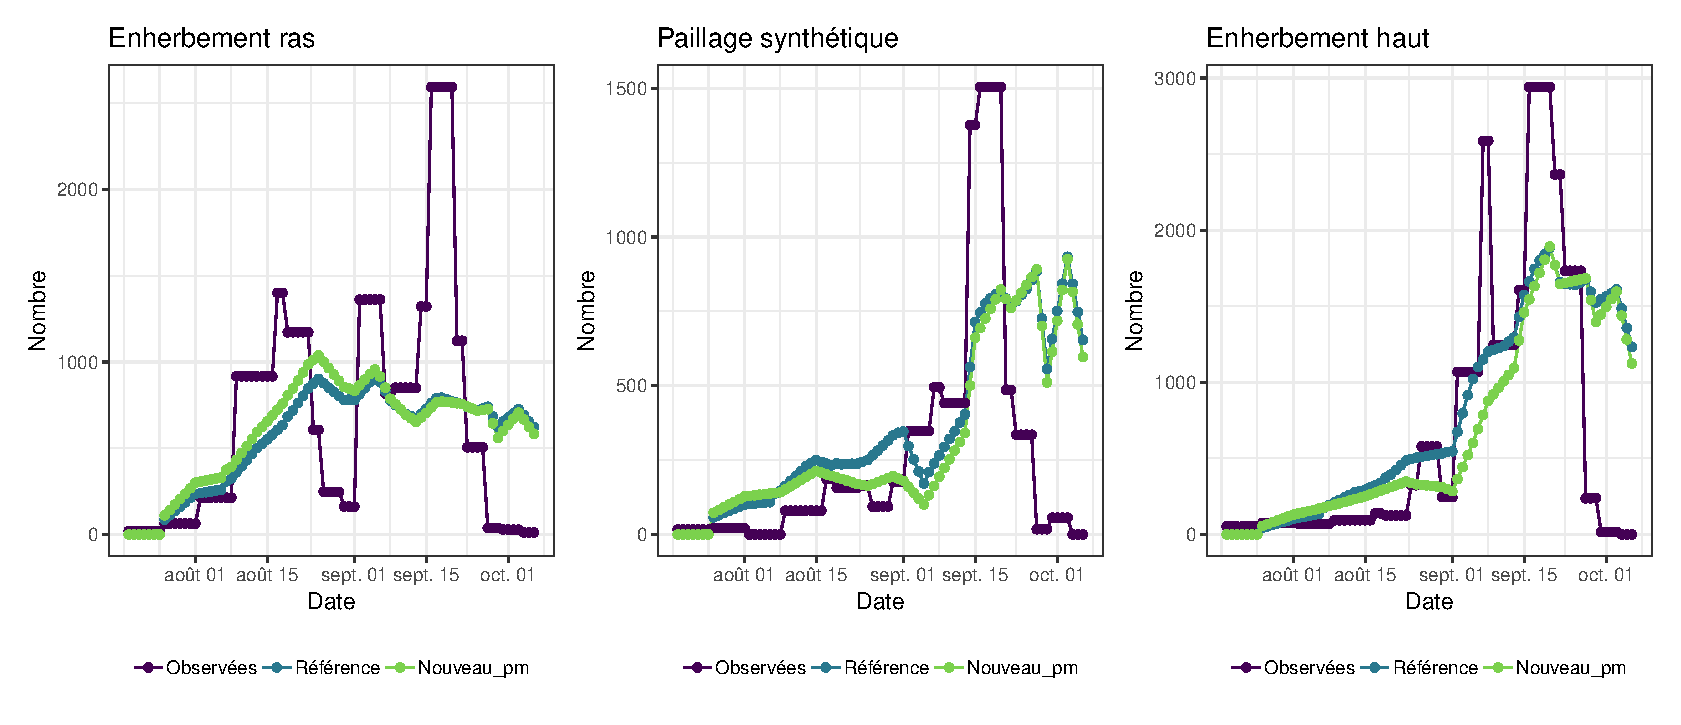
\epsfig{file = plots/pm_v_ref.eps, scale = 0.55}
 \caption{Comparaison de l'ancienne estimation de référence avec l'estimation avec la nouvelle hypothèse sur les échanges intra-bloc.}
 \label{fig:comp}
\end{figure}


\textit{A priori} seulement car lorsque l'on s'intéresse aux paramètres, les différences se font nettes comme le montre les paramètres estimés : 
{%
\newcommand{\mc}[3]{\multicolumn{#1}{#2}{#3}}
\begin{center}
\begin{tabular}{lllll}
\mc{5}{c}{Estimation de référence}\\
$\gamma$ & $p_m$ & $\mu_{ER}$ & $\mu_{EH}$ & $k$\\
0.041 & 0.593 & 0.536 & 0.000 & 62.771\\
\mc{5}{c}{Nouvelle estimation}\\
$\gamma$ & $p_{\text{PS}}$ & $\mu_{ER}$ & $\mu_{EH}$ & $k$\\
0.053 & 0.000 & 0.155 & 0.000 & 68.232
\end{tabular}
\end{center}
}%
On s'aperçoit que les échanges deviennent nuls à l'intérieur du bloc. De plus, il n'y a pas d'émergence de cécidomyies sur la parcelle avec de l'enherbement haut (ce qui était déjà le cas avant). Cela implique que pour le paillage synthétique et l'enherbement haut, le modèle ajuste uniquement avec des individus exogènes. Cela se vérifie sur la figure~\ref{fig:decompo}.



\begin{figure}[ht]
 \centering
 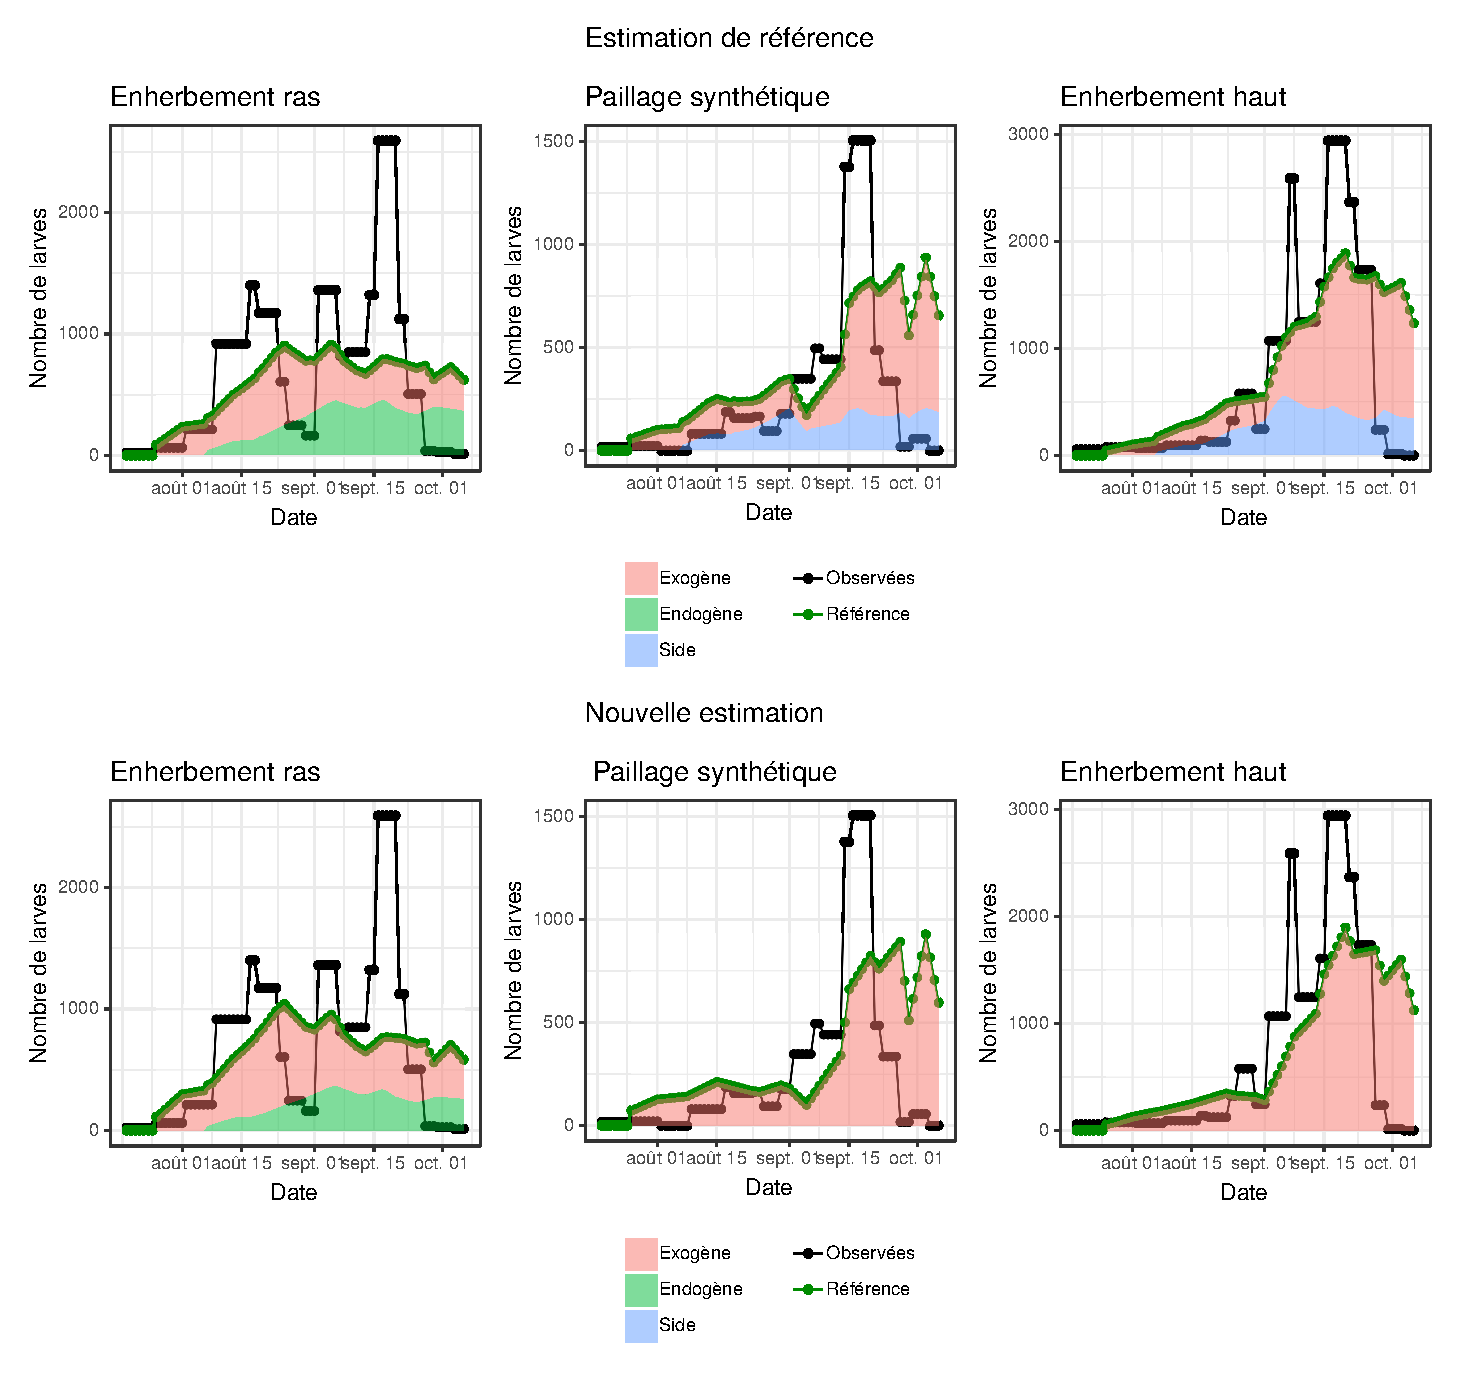
\epsfig{file = plots/decompopo.eps, scale = 0.65}
 \caption{Comparaison la provenance des femelles produisant des larves pour chaun des trois sous-blocs en fonction des deux estimations réalisées.}
 \label{fig:decompo}
\end{figure}







\clearpage
\section{Estimation de référence}

À partir de là, il fut convenu d'établir une nouvelle estimation de référence. Estimation utilisant la nouvelle hypothèse concernant les échanges intra-bloc, la répartition «en cloche» de la durée de larvation et en utilisant les inflorescences attractives simulées en entrée. Cela produit les dynamiques visibles sur la figure~\ref{fig:newref}.

\begin{figure}[ht]
 \centering
 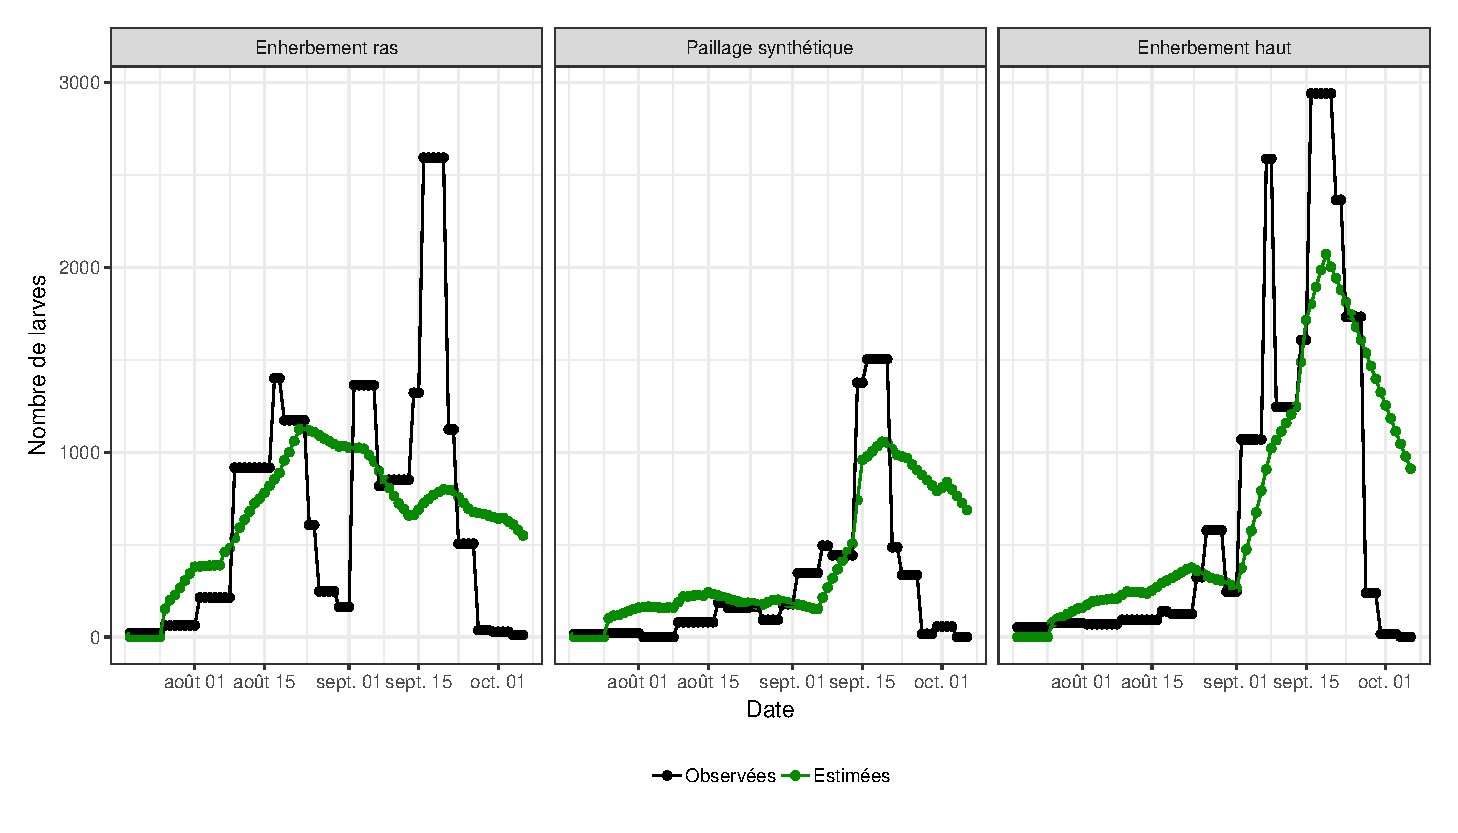
\epsfig{file = plots/new_new_ref.eps, scale = 0.65}
 \caption{Comparaison du nombre de larves observées et estimées pour chacun des trois sous blocs.}
 \label{fig:newref}
\end{figure}

Les paramètres associés sont
\begin{center}
\begin{tabular}{lllll}
$\gamma$ & $p_{\text{PS}}$ & $\mu_{ER}$ & $\mu_{EH}$ & $k$\\
0.073 & 0.373 & 0.223 & 0.000 & 10.788
\end{tabular}
\end{center}

Des échanges entre l'enherbement ras et le paillage synthétique sont présents. En revanche, il n'y a toujours pas d'individus endogènes pour l'enherbement haut.

En guise de conclusion, on peut noter que l'amélioration hypothétique induite par le changement des échanges entre les sous-blocs n'est pas là. On pourrait même dire que c'est une dégradation du modèle dans la mesure où la population de larves de l'enherbement haut ne provient plus qu'exclusivement des femelles exogènes --- il y avait auparavant des femelles provenant de l'enherbement ras.


\end{document}

